% Chapitre 2 - Page 5 | Travaux Avant-Projet | L3 ELN
\documentclass[11pt,a4paper]{article}
\usepackage{fontspec}
\setmainfont{TeXGyrePagella}
\usepackage[french]{babel}
\usepackage{tikz}
\usetikzlibrary{calc}
\usepackage{graphicx}
\usepackage{xcolor}
\usepackage{geometry}
\geometry{margin=0pt}
\pagestyle{empty}
\definecolor{bleufonce}{HTML}{1B3A6B}
\definecolor{bleupale}{HTML}{D9E9FB}
\definecolor{bleuclaire}{HTML}{EAF3FB}
\newcommand{\pos}[4]{\node[anchor=north west,inner sep=0pt,outer sep=0pt,text width=#3,align=left] at ($(current page.north west)+(#1,-#2)$) {#4};}
\newcommand{\sect}[1]{{\color{bleufonce}\bfseries\fontsize{17}{19}\selectfont #1}}
\newcommand{\bodyfont}{\fontsize{10.5}{13.2}\selectfont}
\newcommand{\smallfont}{\fontsize{9.5}{11.5}\selectfont}
\begin{document}
\begin{tikzpicture}[remember picture,overlay]
\path[use as bounding box] (0,0) rectangle (0,0);
\draw[bleufonce,line width=.95pt,rounded corners=8mm]
  ($(current page.north west)+(5mm,-5mm)$) rectangle
  ($(current page.south east)+(-5mm,5mm)$);

% Page de cours : commencer directement sous la bordure, sans en-tête.

% intro line for image
\pos{10mm}{13mm}{188mm}{\sect{Notre exemple sous Proteus}}
\pos{10mm}{26mm}{188mm}{{\bodyfont La figure suivante représente la \textbf{simulation de notre exemple} réalisée sur \textbf{Proteus}. Elle correspond à l'exemple fil rouge étudié dans ce chapitre.}}

% image frame
\begin{scope}[shift={($(current page.north west)+(18mm,-44mm)$)},x=1mm,y=-1mm]
  \draw[bleufonce,line width=.75pt,rounded corners=2mm] (0,0) rectangle (174,79);
  \node[anchor=north west,inner sep=1.5mm] at (2.1,1.5) {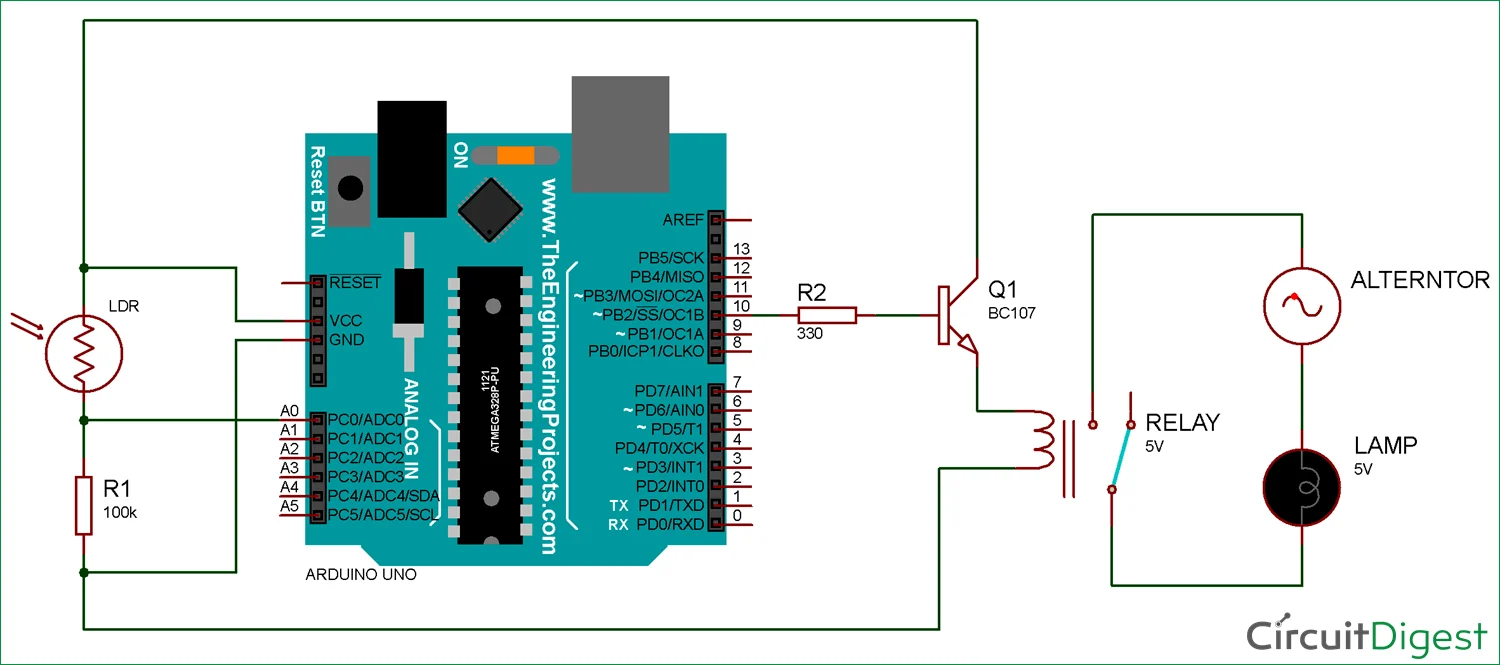
\includegraphics[width=170mm,height=76mm,keepaspectratio]{assets/chap2_page5_proteus_example.png}};
\end{scope}
\pos{20mm}{127mm}{170mm}{{\color{bleufonce!80}\smallfont Figure --- Simulation de l'exemple du chapitre sous Proteus.}}

% tinkercad section
\pos{10mm}{140mm}{188mm}{\sect{4. Découvrir Tinkercad}}
\pos{10mm}{153mm}{188mm}{{\bodyfont Tinkercad est une plateforme simple et accessible qui permet de créer des montages électroniques virtuels. Elle est surtout utilisée pour la découverte de \textbf{l'Arduino}, du \textbf{breadboard} et de la programmation de base. Son interface est claire, ce qui la rend adaptée à l'apprentissage et aux premières manipulations.}}

\pos{10mm}{185mm}{188mm}{\sect{Ce que l'on trouve dans Tinkercad}}
\pos{16mm}{198mm}{181mm}{{\bodyfont
\textcolor{bleufonce}{\textbullet}\enspace Une zone de travail pour placer les composants.\\[2.2mm]
\textcolor{bleufonce}{\textbullet}\enspace Des cartes comme \textbf{Arduino Uno}.\\[2.2mm]
\textcolor{bleufonce}{\textbullet}\enspace Des composants de base : LED, résistances, boutons, potentiomètres, capteurs simples, buzzer, etc.\\[2.2mm]
\textcolor{bleufonce}{\textbullet}\enspace Un espace pour écrire et tester un programme Arduino.\\[2.2mm]
\textcolor{bleufonce}{\textbullet}\enspace Une simulation visuelle proche du montage réel.
}}

% note box
\draw[bleufonce,line width=.8pt,rounded corners=2.8mm]
  ($(current page.north west)+(10mm,-241mm)$) rectangle
  ($(current page.north west)+(200mm,-271mm)$);
\pos{16mm}{246mm}{174mm}{{\color{bleufonce}\bfseries\fontsize{12}{14}\selectfont Remarque importante}}
\pos{16mm}{255mm}{174mm}{{\fontsize{9.2}{10.7}\selectfont Tinkercad propose une simulation visuelle proche de la réalité, mais \textbf{de nombreux composants ne sont pas disponibles}. La page suivante présente son interface.}}

% footer
\draw[bleufonce!55,line width=.45pt] ($(current page.south west)+(10mm,14.7mm)$) --
  ($(current page.south east)+(-10mm,14.7mm)$);
\node[anchor=south west,inner sep=0pt,text=bleufonce!80] at ($(current page.south west)+(10mm,7.4mm)$)
  {\fontsize{9.5}{11}\selectfont 2026/2027};
\node[anchor=south east,inner sep=0pt,text=bleufonce!80] at ($(current page.south east)+(-10mm,7.4mm)$)
  {\fontsize{9.5}{11}\selectfont Page 5};
\end{tikzpicture}
\null
\end{document}
